\documentclass[hyperref={pdfpagelabels=false},usepdftitle=false]{beamer}
\usepackage{../templates/myStyle}

\begin{document}
\selectlanguage{ngerman}

\title{\titleText}
%\subtitle{Pixelweise Klassifikation von Straße}
\author{\tutor}
\date{17. Juni 2015}
%\subject{Programmieren}

\frame{\titlepage}

\frame{
    \frametitle{Contents}
    \setcounter{tocdepth}{1}
    \tableofcontents
    \setcounter{tocdepth}{2}
}

%\AtBeginSection[]{
%    \InsertToC[sections={\thesection}]  % shows only subsubsections of one subsection
%}

%!TEX root = Zwischen-ML-Prak-2015.tex
\section{Worum es geht}

\subsection{Die Aufgabe}

\begin{frame}{Die Aufgabe}
    \begin{itemize}
        \item \textbf{Eingabe}: Bilder, die von einer Kamera aus Fahrersicht
              aufgenommen wurden
        \item \textbf{Ausgabe}: Ein Bild gleicher Größe, wo jedes Pixel
              entweder schwarz ist (wenn der Klassifikator denkt es ist Straße)
              oder weiß ist (wenn dem) nicht so ist.
    \end{itemize}
\end{frame}

\begin{frame}{Die Daten}
    \href{http://www.cvlibs.net/datasets/kitti/eval_road.php}{KITTI Road Estimation dataset}
    \begin{itemize}
        \item Daten-Bilder der Größe $[1226, \dots, 1242] \times [370, \dots, 376]$,
              8-bit RGB
        \item Label-Bilder der selben Größe; 8-bit RGB mit 2 Farben
        \item 289 Trainingsbilder
        \item 290 Testbilder
    \end{itemize}
\end{frame}

\framedgraphic{Daten}{../images/umm_000000.png}
\framedgraphic{Labels}{../images/umm_road_000000.png}
\framedgraphic{Overlay}{../images/um_000000-overlay.png}
%!TEX root = Zwischen-ML-Prak-2015.tex
\section{Paper}

\subsection{Paper}

\begin{frame}{Paper}
    \begin{itemize}
        \item \href{http://arxiv.org/abs/1411.4038}{Fully Convolutional Networks for Semantic Segmentation}:
              Jonathan Long, Evan Shelhamer, Trevor Darrell
        \item pixelwise segmentation of multiple classes
    \end{itemize}
    
   
\end{frame}

\framedgraphic{Paper - Results}{../images/paper_results.png}
\framedgraphic{Paper - Heatmap}{../images/paper_heatmap.png}
\framedgraphic{Paper - Deconvolution}{../images/paper_dc.png}

%!TEX root = Zwischen-ML-Prak-2015.tex
\section{Lessons learned}

\subsection{Caffe}

\begin{frame}{Erste Ergebnisse}

\centering

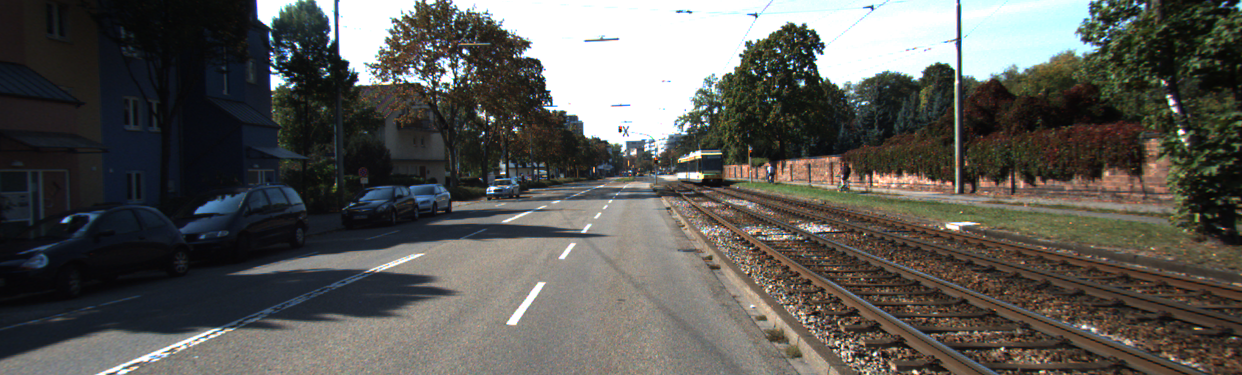
\includegraphics[width=0.75\textwidth]{../images/umm_000000.png}

\hspace{0.5cm}

\only<1>{

\includegraphics[width=0.75\textwidth]{../images/um-segmentation.png}
}

\only<2>{
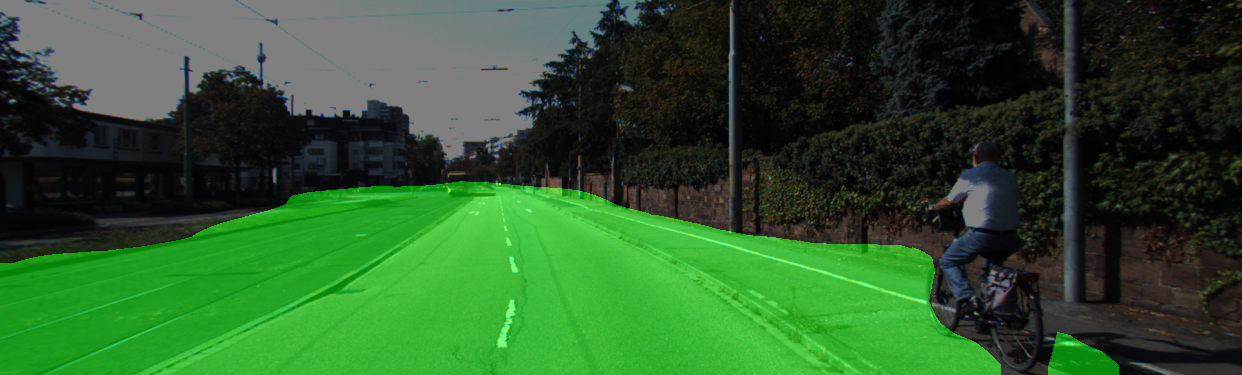
\includegraphics[width=0.75\textwidth]{../images/um-overlay.png}
}

 %TODO: Komische Fehler (TODO: ein paar einbinden)

\end{frame}

\begin{frame}{Challenges}

\centering

\begin{itemize}
 \item Reduziere Netzgröße (von 11.5 GiB) \\
 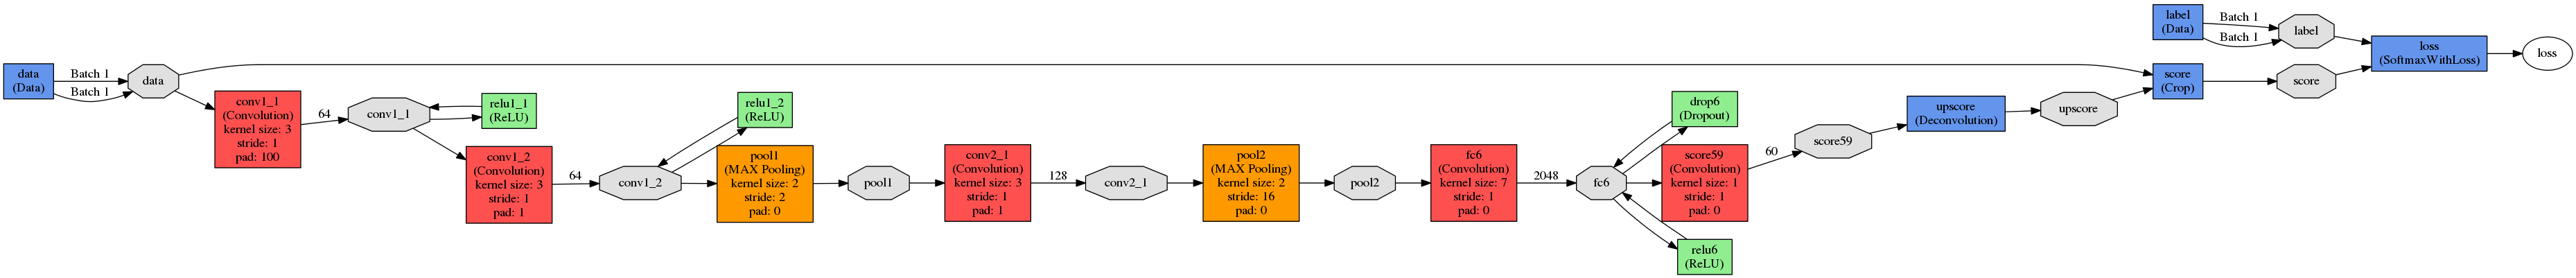
\includegraphics[width=0.9\textwidth]{../images/mid.png}
 \item trainiere mit Eigenen Daten \\
 \begin{minipage}{0.45\textwidth}
 
\includegraphics[width=\textwidth]{../images/out.png}
 \end{minipage}  \begin{minipage}{0.45\textwidth}
 
\includegraphics[width=\textwidth]{../images/out-um.png}  
 \end{minipage}
\end{itemize}
\end{frame}
%!TEX root = Zwischen-ML-Prak-2015.tex
\section{Sliding Window}

\subsection{Sliding Window}

\begin{frame}{Sliding Window}
  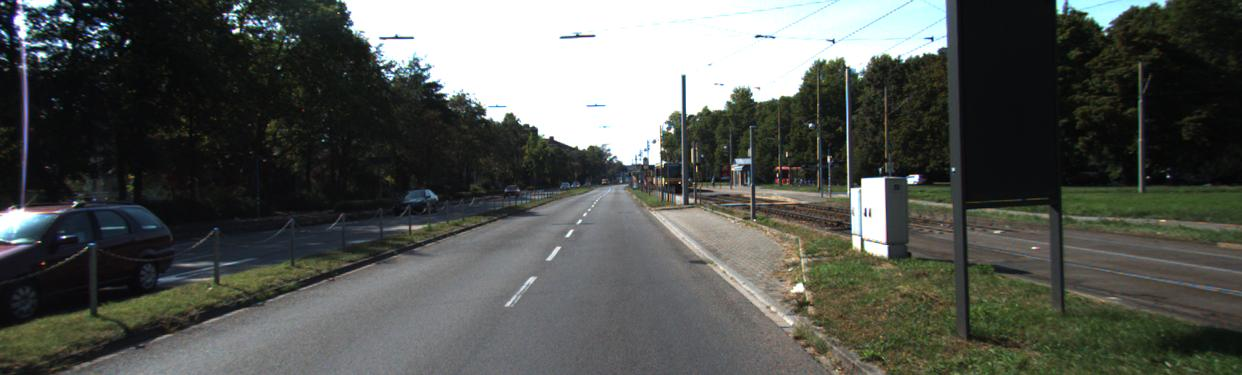
\includegraphics[scale=0.11]{../images/Lasagne/padded.jpg}
  \hspace{0.1cm}
      
\includegraphics[scale=0.12]{../images/Lasagne/29x29-color-coordinates.jpg}
         \vspace{0.1cm}
    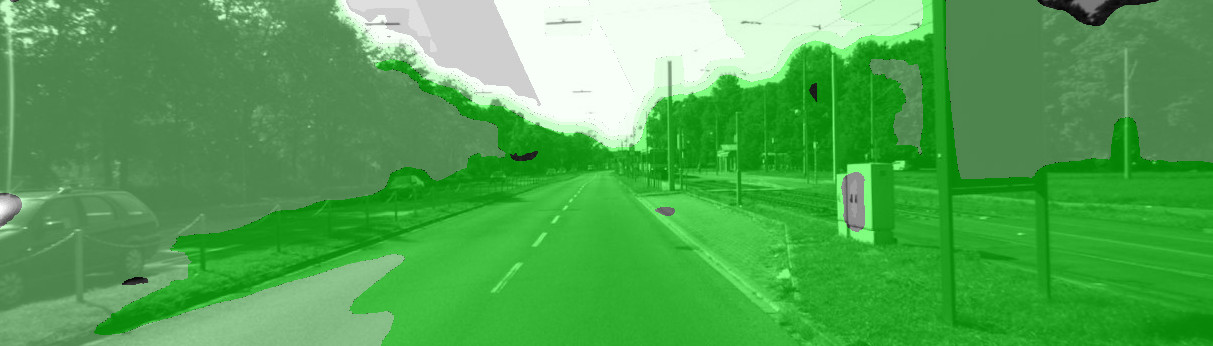
\includegraphics[scale=0.2]{../images/Lasagne/29x29-color-coordinates-overlay.jpg}
         \begin{itemize}
       \item Implementierung mit Lasagne, Windowsize 29~Pixel
        \item Pixelkoordinate als zusätzliches Feature
    \end{itemize}
  $\rightarrow$ \emph{schlechte Ergebnisse}, \emph{lange Laufzeit}

\end{frame}

\section{Ausblick}
\subsection{Ausblick}
\begin{frame}{Ausblick}
    \begin{itemize}
        \item Siliding Window Ansatz nicht weiterverfolgen
        \item in Kontakt mit Jonathan Long, bzgl. Caffe Implementierung
        \item Fully Concolutional Networks mit Lasagne implementieren
    \end{itemize}
    Davon erhoffen wir uns:
    \newline
    $\rightarrow$ \emph{flexible Anpassung},  \emph{schnellere Laufzeit} und  \emph{gute Resultate}
\end{frame}
%!TEX root = Zwischen-ML-Prak-2015.tex
\section*{End}
\subsection{End}
% \subsection{Sources}
% \begin{frame}{Image Sources}
%     \begin{itemize}
% 	\item \href{https://commons.wikimedia.org/wiki/File:Server-multiple.svg}{Server} by RRZEicons
%     \item \href{https://commons.wikimedia.org/wiki/File:Computer-aj_aj_ashton_01.svg}{Desktop Computer} by Ed g2s,
%           Ironbrother, Kierancassel and Msgj
%     \item \href{https://commons.wikimedia.org/wiki/File:Server_by_mimooh.svg}{Server} by Mimooh
%     \end{itemize}
% \end{frame}

\framedgraphic{Thanks for Your Attention!}{../images/um_000000.png}

\end{document}
